\documentclass{article}
%
%\usepackage{pdfsync}           % Used in Mac OSX
\usepackage[mathcal,mathbf]{euler}
\usepackage{theorem,amsmath,enumerate,fancyhdr,amssymb,amsfonts}
\usepackage{graphicx}           %Used in Mac OSX
%\usepackage[pdftex]{graphics}  %Might be needed in non Mac OSX systems
\usepackage{myDefs}
\usepackage{url}
%In order to be consistent use the following notation in your notes:

\title{
ISH data interaction matrix analysis
}
\author{Avinash Das}

\date{\today}
\begin{document}

\pagestyle{fancy}
\lhead{{\bf Avinash Diary}{ }
\\{\bf } } 
\rhead{{\bf Date: }\today}

\maketitle

\section{Initial Analysis}
I performed some initial analysis on the sample interaction data present at \url{http://www.eurexpress.org/ee/tools/EurExpressCluster_01.zip}.
At first, I tested whether there are certain classes of genes those are expressed in different anatomy ( those are significantly more than expected, like the housekeeping genes analysis similar to \cite{eisenberg2003human}). Figures ~\ref{fig:strongHist} , \ref{fig:mildlyHist} and \ref{fig:weaklyHist} respectively shows the histogram of strongly expressed, mildly expressed ( genes those are highly or mildly expressed) and weakly expressed genes ( highly, mildly or weakly expressed).  
I have also overlay corresponding null distribution for each of the cases. I assumed binomial distribution with mean equal to observed mean as the null distribution. 
As seen from the figure the class genes are significantly compared to null distribution, particular in (1) classes where a gene is expressed in fewer number of anatomies (Probably this is not very interesting). (2) classes where a gene is expressed many tissues. 

\begin{figure}
	\begin{center}
		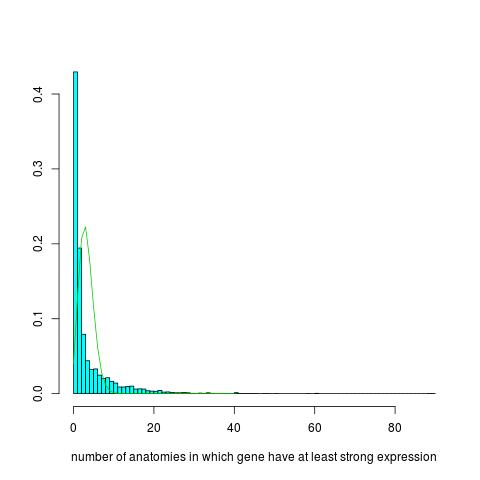
\includegraphics[scale=0.5]{../../data/strongExpressed.jpg}
	\end{center}
	\caption{Strongly expressed  gene histogram }
	\label{fig:strongHist}
\end{figure}

\begin{figure}	
	\begin{center}
		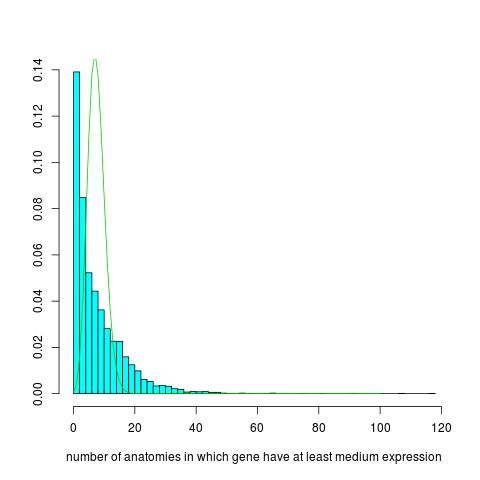
\includegraphics[scale=0.5]{../../data/midlyExpressed.jpg}
	\end{center}
	\caption{mildly expressed gene histogram}
	\label{fig:mildlyHist}
\end{figure}

\begin{figure}
	\begin{center}
		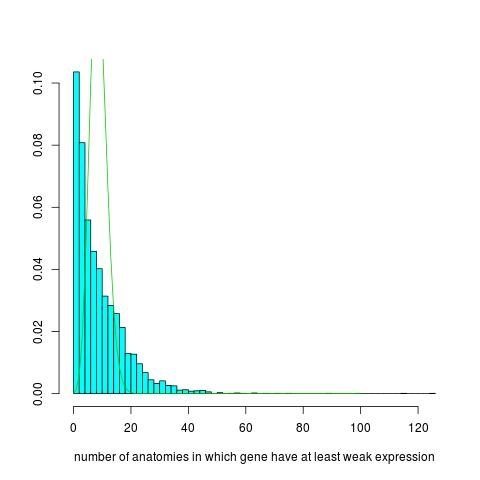
\includegraphics[scale=0.5]{../../data/weaklyExpressed.jpg}
	\end{center}
	\caption{weakly expressed gene histogram}
	\label{fig:weaklyHist}
\end{figure}

Next, I performed some annotation analysis whether these over represented genes are enriched in any particular annotation. I further divided the genes which are strongly expressed in many anatomies (and occur more than expected by null distribution P-value $<$ E-8) into following groups:
\begin{itemize}
	\item Strong40: The genes which are strongly expressed in more than 40 anatomy are enriched in membrane
		related annotation. The annotation have two prominent clusters: one with membrane and trans-membrane function; other with bi-sulfide  related functions.
	\item  Stong20: The genes which are strongly expressed in more than 20 anatomy are enriched in homestatis, adhesion and DNA repair functions,
		in addition to membrane and bi-sulfide functions.
	\item  Strong8: The genes which are strongly expressed in more than 8 anatomy are enriched in growth factor activity, glycoprotien and muscle 
		development
		in addition to functionalities of strong40 and strong20.
\end{itemize}


It seems the genes, which are strongly expressed across many anatomies, are enriched in house-keeping functions (note I have reported only those annotation clusters which
are significantly compared to all mouse genes as background). 




\bibliographystyle{apalike}	% (uses file "plain.bst")
\bibliography{diary}		% expects file "myrefs.bib"

\end{document}
